\documentclass[tikz]{standalone}

\usetikzlibrary{arrows}
\usetikzlibrary{arrows.meta}

\begin{document}

\begin{tikzpicture}[baseline=-0.5ex,scale=2.0]
    % create a white background, with a black frame
    % \draw [fill=white] (-3,-0.5) rectangle (3,0.5); 
    \draw[thick,->] (-2.5,0) -- (2.5,0);
    
    \node at (-2,0.2) {\Large $-$};
    \node at (-0.5,0.2) {\Large $+$};
    \node at (0.5,0.2) {\Large $-$};
    \node at (2,0.2) {\Large $+$};
    
    \foreach \x in {-1,0,1} 
        \draw [thick] (\x cm,2pt) -- (\x cm,-2pt) node[below] {$\x$};
\end{tikzpicture}

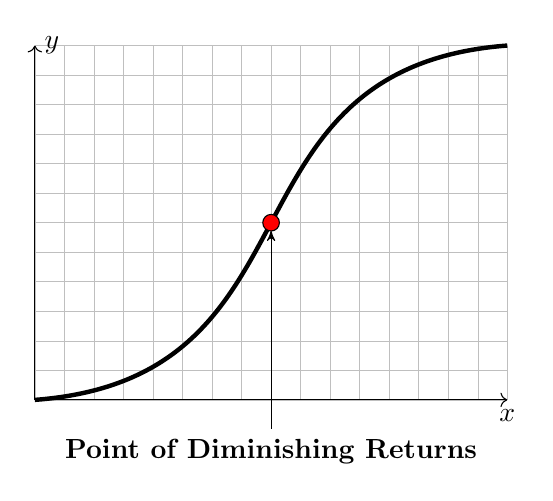
\begin{tikzpicture}[scale = 1.5]
    % \draw[white,fill=white] (0,0) rectangle (4,3);
        %\draw[very thin,color=darkgray,step=1.0] (0,0) grid (4,3);
        \draw[very thin,color=lightgray,step=0.25] (0,0) grid (4,3);
    
    \draw[->] (0,0) -- (4,0) node[below] {$x$};
    \draw[->] (0,0) -- (0,3) node[right] {$y$};
            
    % draw curve
    \draw [ultra thick] (0,0) .. controls (2.5,0.1875) and (1.5,2.8125) .. (4,3);
    
    % draw points
    \draw [black,fill=red] (2,1.5) circle (2.0pt);
    
    % label extrema
    \draw [<-, >=stealth', shorten <=3pt] (2,1.5) -- (2,-0.25) node[below] {\bf Point of Diminishing Returns}; 
    
\end{tikzpicture}

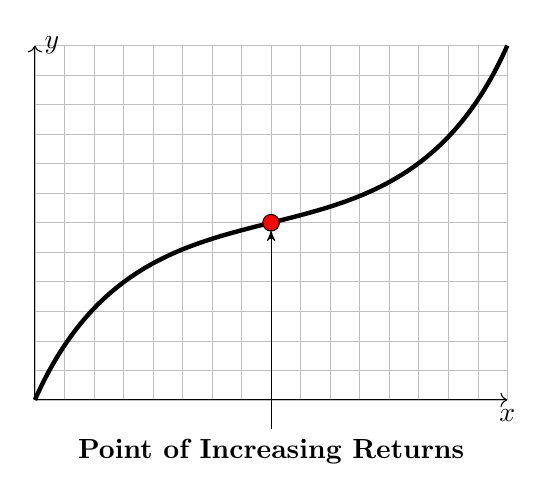
\begin{tikzpicture}[scale = 1.5]
    
    % \draw[white,fill=white] (0,0) rectangle (4,3);
        %\draw[very thin,color=darkgray,step=1.0] (0,0) grid (4,3);
        \draw[very thin,color=lightgray,step=0.25] (0,0) grid (4,3);
    
    \draw[->] (0,0) -- (4,0) node[below] {$x$};
    \draw[->] (0,0) -- (0,3) node[right] {$y$};
    
    
    % draw curve
    \draw [ultra thick] (0,0) .. controls (1,2.25) and (3,0.75) .. (4,3);
    
    % draw points
    \draw [black,fill=red] (2,1.5) circle (2.0pt);
    
    % label extrema
    \draw [<-, >=stealth', shorten <=3pt] (2,1.5) -- (2,-0.25) node[below] {\bf Point of Increasing Returns}; 
    
\end{tikzpicture}

\begin{tikzpicture}[baseline=-0.5ex,scale=1.5]
    \draw[thick,->] (0,0) -- (4,0);
    
    \node at (1,0.2) {\Large $-$};
    \node at (3,0.2) {\Large $+$};
    
    \foreach \x in {2} 
        \draw [thick] (\x cm,2pt) -- (\x cm,-2pt) node[below] {$\x$};
\end{tikzpicture}

\end{document} 